\subsection{תיקון מסדר שני עבור $\mathbf{l=1}$}
הפעם כדי לפתח את זה נצטרך לחזור לצורה הנוכחית של משוואה (4). כעת עם $l=1$ אנחנו מקבלי איבר נוסף בפוטנציאל האפקטיבי ומשוואה (4) מקבלת את הצורה
$$-\frac{1}{2}u''(r)+\left(-\frac{Z}{r} + \frac{1}{r^2}\right)u(r)=\epsilon u(r)$$
כאשר נציב את הפיתוח טיילור של $u$ סביב $r=0$ נקבל
$$-\frac{1}{2}\left(u''_0+u^{(3)}_0r + O(r^2)\right)+\left(-\frac{Z}{r} + \frac{1}{r^2}\right)\left(u'_0r+\frac{u''_0}{2}r^2 + O(r^3)\right)=\epsilon \left(u'_0r + O(r^2)\right)$$
כשנסתכל על המקדמים של $r^0$ נקבל את המשוואה $-u''_0/2-Zu'_0+u''_0/2=0$ כלומר $u'_0=0$. 
נסתכל על $u_1$ כפיתוח טיילור כמו שעשינו בפעמים הקודמות.
$$u_1=u'_0\Delta+u''_0\Delta^2 + O(\Delta^3) \approx u''_0\Delta^2$$
כלומר 
$$u''_0 = \frac{2}{2\Delta^2}u_1 \quad\Rightarrow\quad H^{(2)}_{11} = H_{11} + \frac{1}{12}\frac{1}{\Delta^2}$$
נשים לב שהתיקוןוב מסדר ראשון שלו נופל ונשארים עם תיקונים מסדר שני ומעלה. תוצאה זו מתאימה לכך שעבור $l$ גדול יותר ההתכנסות הייתה יותר מהירה.
נשווה בין התוצאות עם התקון לתוצאות ללא התיקון
\begin{figure}[h!]
    \begin{minipage}[t]{0.45\textwidth}
        \centering
        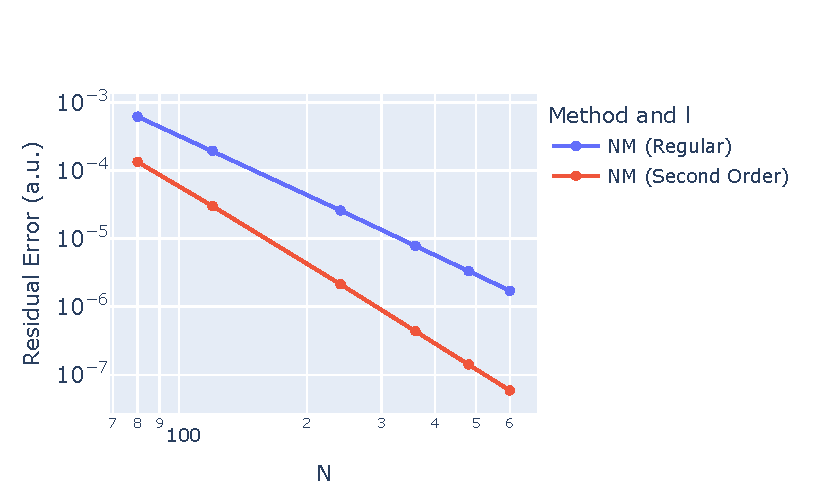
\includegraphics[width=\linewidth, trim=0 0 0 1cm, clip]{plots/second_order_l1/residual_error.eps}
        \caption{השגיאה השיורית השוואה בין המצב ללא תיקון, ותיקון מסדר שני עבור $l=1$}
        \label{fig:second_order_residual_error}
    \end{minipage}
    \hfill
    \begin{minipage}[t]{0.45\textwidth}
        \vspace{-2cm}
        \centering
        \begin{tabular}{c c}
תיקון & $q$ \\
\hline
ללא תיקון & $2.85738$ \\
תיקון מסדר שני & $3.68646$ \\
\end{tabular}

        \captionof{table}{קצב ההתכנסות עבור רמות התיקון השונות עבור $l=1$}
        \label{tab:second_order_convergence_rates}
    \end{minipage}
\end{figure}
